\documentclass{article}
\usepackage[utf8]{inputenc}
\usepackage{graphicx}

\title{Expos\'{e} Master Thesis\\
  Rollup System for Layer 2 Scaling}
\author{Thi Thu Ha Doan \and  Peter Thiemann}
\date{December 2022}

\begin{document}

\maketitle

\section{Introduction}
Blockchain systems have grown rapidly in recent years. However, the increased activity has come at a cost to the use of the network. Many blockchains have reached their capacity limits. The high demand on the network slows down transactions and increases gas prices, so a "scaling solution" is needed and becomes an urgent problem. The main goal of scalability is to increase transaction speed and throughput while ensuring decentralization and security.

Various scaling solutions have been proposed by both industry and academic communities. The solutions can be divided into two catalogues: first layer and second layer scaling solutions. The first layer scaling solutions (on-chain scaling) require changes to the blockchain protocol. For this solution, we can mention Proof-of-stake protocol and Sharding. Second layer scaling (off-chain scaling)  uses a separate network called layer 2 (L2) that runs on top of the main layer 1 (L1) network and derives the security guarantee from the main network. Current second layer scaling solutions include: State Channels, Sidechain, Plasma and Rollup.

Rollups are an off-chain scaling solution that reduces computational overhead in the main network by moving computation and storage off-chain to L2. Rollup systems inherit the security of the mainnet by publishing computation results on the chain, as shown in Fig~\ref{rollup-batch}. Rollups process a large number of transactions in a rollup batch and then send the compressed summary data defining the changes to the system state to L1. This approach allows fixed costs to be spread across multiple transactions in each rollup batch, reducing user charges. Rollups therefore provide a significant improvement in transaction throughput.

\begin{figure}[t]
\caption{Rollup systems}
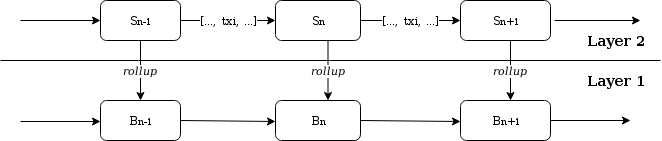
\includegraphics[width=12cm]{rollup-batch}
\label{rollup-batch}
\centering
\end{figure}

The goal of this work is to investigate the efficiency of the rollup scaling solution for the blockchain scaling problem. This work aim to explain the rollup technology in depth.  We design and implement a prototype of  rollup systems that covers all the main architects of a rollup system, but keeps it as the core system.

\section{Design and Implementation of a Prototype for Rollup Systems}
In rollup systems, users sign transactions and submit them to an aggregator (sequencer) that checks, orders, and executes these transactions. The aggregator then compresses the data into a rollup batch and compresses the batch with other necessary data (e.g., system state ) into a rollup block and publishes that rollup block as a single transaction on L1. There are two different ways to publish the data to the network. The first approach is optimistic rollup, which assumes that the off-chain transactions are valid and does not require validity proofs for the off-chain transactions in the rollup batch. Another approach is zero-knowladge rollup (ZK rollup), in which the aggregator must publish proofs of validity. In contrast, an optimistic rollup responds to a fraud proof to determine where transactions are invalid. After a rollup batch is submitted to L1, anyone can challenge the results of a rollup transaction by computing a fraud proof.

We tend to keep the prototype pure. The implementation contains only the core components of a rollup system, but is capable of extending the system if we want to enrich it for future research. For security, the system relies on a fraud detection procedure as in optimistic rollups. A fraud proof is an assertion that a state transition is invalid and therefore the entire batch should be reversed. The prototype targets the Etherum blockchain, which is the second largest blockchain and has an urgent "scaling problem." The architect of the prototype rollup system is shown in Fig~\ref{rollup-design}.

\begin{figure}[t]
\caption{Design of the rollup system}
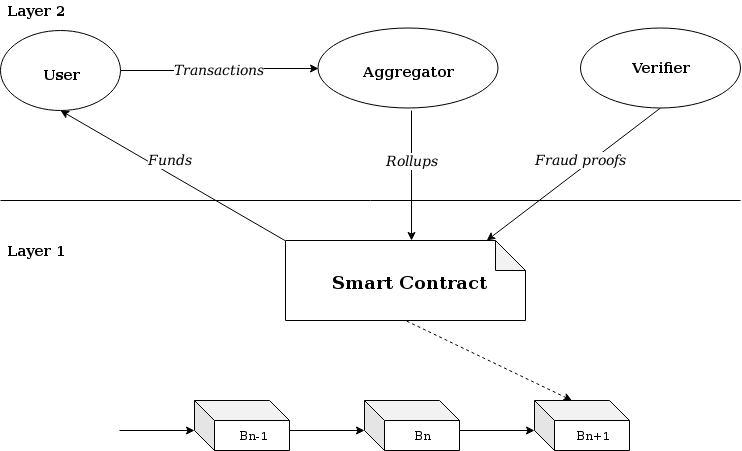
\includegraphics[width=12cm]{rollup-design.png}
\centering
\label{rollup-design}
\end{figure}

\subsection{Interacting with the main network}
The operation of the rollup system is controlled by a smart contract deployed on-chain. The L2 system interacts with L1 through the smart contract. The contract receives and processes rollup blocks. It also stores and updates the status of the rollup system and tracks user deposits. In addition, the contract provides functions to verify rollup batches in the challenge period. Users must deposit money into the smart contract before they can use the system. The money is then locked in the contract and the user receives a corresponding amount that can be used in the rollup system.

\subsection{Submitting rollup batches}
The aggregator receives transactions signed and sent by users. In a rollup system, a transaction may come from a user in L2 via a direct peer-to-peer network or from L1 via an intermediate contract running on L1. However, in this prototype rollup system, for simplicity, only transactions that are transmitted by and originate from users in L2 are offered. After the aggregator receives the transactions from users, it verifies, orders, and executes them. The aggregator then bundles the off-chain transactions into a rollup batch and sends it to L1 via the smart contract call. In this process, the transaction data is compressed and published on-chain as call data. The published data contains the system state root and the transaction stack in a rollup block in a highly compressed form. Since the calldata is on-chain as part of the history logs, but not stored in the smart contract, it is less expensive.

A system state constructed as shown in  Fig~\ref{rollup-batch-data} is a term that refers to the available information about the rollup system at a given time. The state includes key information about the network such as accounts, balances, etc. It is organized as a Merkle tree and the root of this tree is the state root, which refers to the last state of the rollup system. Each state transition in the chain results in a new rollup state, which the aggregator determines by computing a new state root. This root state is hashed, sent, and stored in the on-chain smart contract. The aggregator must transmit both the previous and new state roots when it publishes the rollup batches. If the previous state root matches the existing state root in the smart contract, the latter is discarded and replaced with the new state root (post state root).

\subsection{Data availability}

Since a malicious aggregator can steal funds by publishing invalid transactions and root state, the security of the system relies on an honest verifier re-executing transactions in a rollup batch and submitting fraud proofs to challenge invalid state transitions. Since on-chain execution is based on submitted transaction-related data, anyone can use this information to execute rollup state and verify the correctness of state transitions. Therefore, data availability is critical because without access to the state data, the verifier cannot create fraud evidence to dispute invalid rollup batches. Therefore, all required transaction information must be published in L1 so that these transactions can be re-executed when needed.

However, if the full transaction data is published as calldata on the mainnet, this could be expensive. Therefore, the rollup system uses compression techniques to reduce the amount of transaction-related data. Compression of the data is achieved by publishing only the information required to deterministically re-execute the transaction. The batch of these transactions in compressed form is published on the chain as call data for the smart contract.
\begin{figure}[t]
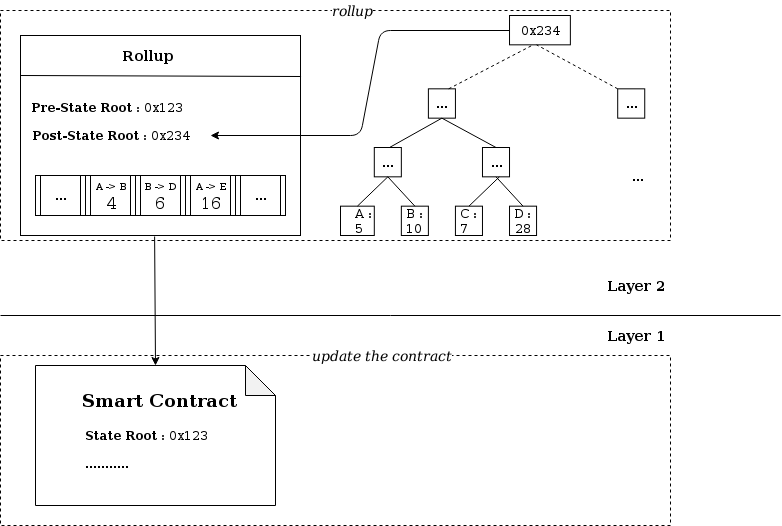
\includegraphics[width=12cm]{rollup-batch-data}
\centering
\label{rollup-batch-data}
\end{figure}
\subsection{Dispute period}
The system allows the aggregator to publish rollup batches without providing proof of validity. However, to prevent any misbehaviour by the aggregator, the rollup system proposes a period of time, called the challenge period, during which anyone can challenge a state transition. This actor is called a verifier in our model. Note that when rollup batches are published on L1, the aggregator must deposit a certain amount of funds that is locked until the end of the challenge period. Similarly, the verifier must lock the same amount as the aggregator if it wishes to challenge the aggregator.

When a verifier initiates the dispute process by submitting a fraud proof claiming that a state transition is invalid and therefore the entire batch should be reversed, the system reruns the transactions in the rollup batch on the master chain to calculate the post-root state that determines who wins the challenge. If this root state is different from the one specified by the aggregator, the aggregator is penalised. As a result, half of the aggregator's deposit is transferred to the verifier and the other half is burned. If the verifier  fails to prove the aggregator's misconduct, the same will happen to the verifier's deposit.

\section{Tasks}
\subsection{Survey of current rollup technologies}
\begin{itemize} 
\item Optimistic rollups. 
\item ZK rollups. 
\item The efficiency of rollups for Layer 2 scaling.
\end{itemize}
\subsection{Investment technologies}
\begin{itemize} 
\item The state tree and state root. 
\item Data compression: various techniques for compressing transaction data. 
\item Dispute progress.
\end{itemize}
\subsection{development of rollup system}
\begin{itemize} 
\item Design, code, and deploy the smart contract on the chain. 
\item Implement the layer 2 system. 
\item Develop the interface for interaction between L1 and L2.
\end{itemize}
\end{document}